\documentclass[11pt,letterpaper]{article}
\usepackage[latin1]{inputenc}
\usepackage{amsmath}
\usepackage{amsfonts}
\usepackage{amssymb}
\usepackage{graphicx}
\usepackage{bm}
\usepackage[margin=1in]{geometry}
\author{Kevin Smith}
\begin{document}
	
	\section{Simulation Results}
	
	Both the feedback control and the periodic control were tested against a historic dataset in a MATLAB simulation. The transition matrix approach was used to generate a transition model from one week of location data of a single fish off the shore of Catalina Island. The fish's behavior during this time was highly periodic, as shown in Figure \ref{fig:periodicFish}. Using this transition model, 100 fish were simulated, and a varying number of AUVs were also simulated using either the feedback control or the periodic control to track this population.
	\\\\
	To evaluate the control, we used three error metrics:
	\begin{enumerate}
		\item
		\textbf{Closest AUV Distance} The Closest AUV Distance error tracked the distance from each simulated fish to the closest AUV, averaged across all of the fish and all time steps of the simulation.
		\item
		\textbf{Fraction In Range} The Fraction In Range metric tracked the fraction of the simulated fish within some distance of an AUV. Since acoustic tracking is only feasible if the AUV is within a certain range of the tag, this error is useful in determining how many fish would have been lost during a track.
		\item
		\textbf{Population Density Error} Population Density Error is a measure between 0 and 1 quantifying the difference between the distribution of simulated fish across the nodes and the distribution of AUVs. For a fish density $\bm p_{\rm fish}$ and AUV density $\bm p_{\rm AUV}$, this error is calculated as
		\[
			e = \sqrt{ \frac 1 2 \left( \bm p_{\rm fish} - \bm p_{\rm AUV} \right) \cdot \left( \bm p_{\rm fish} - \bm p_{\rm AUV} \right) }
		\]
		For this analysis, $\bm p_{\rm AUV}$ is measured from the AUVs' destination nodes; i.e., from the nodes the AUVs are moving towards rather than the nodes to which they are closest at the time.
	\end{enumerate}
	
	\begin{figure}
		\centering
		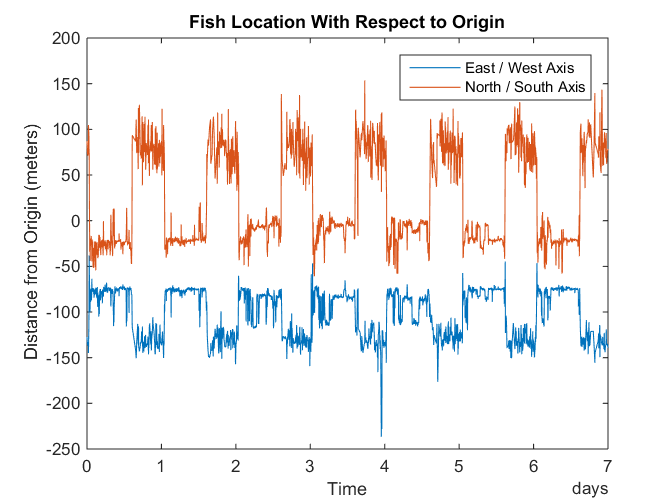
\includegraphics[width = 0.7\linewidth]{results/location}
		\caption{Simulations used a transition model generated from a historical week-long track of a single fish. The above graph shows the fish's coordinates along the East-West and North-South axes from a constant origin.}
		\label{fig:periodicFish}
	\end{figure}
	
	\subsection{Periodic Control}
	
	The periodic control was simulated varying the number of Fourier components kept and the number of AUVs simulated. Since the week of historical data contained 5,040 samples, the resulting transition probability functions contained 2,520 frequency components revealed by an FFT. The periodic control was testing by keeping various numbers of the highest-magnitude frequency components, between 0 (resulting in the AUVs taking random transitions) and 2,520 (in which case the AUVs follow exactly the same transition probabilities as the fish). Also, varying numbers of AUVs, between 1 and 100, were tested.
	\\\\
	Figure \ref{fig:periodicMeanDistance} shows the Closest AUV Distance error for each of the combinations of parameters. As would be expected, when more AUVs are present, fish are more likely to be close to an AUV. When 10 or more AUVs are used, i.e., when there are more AUVs than nodes, even random transitions result in an error below 12 meters. 
	\begin{figure}
		\centering
		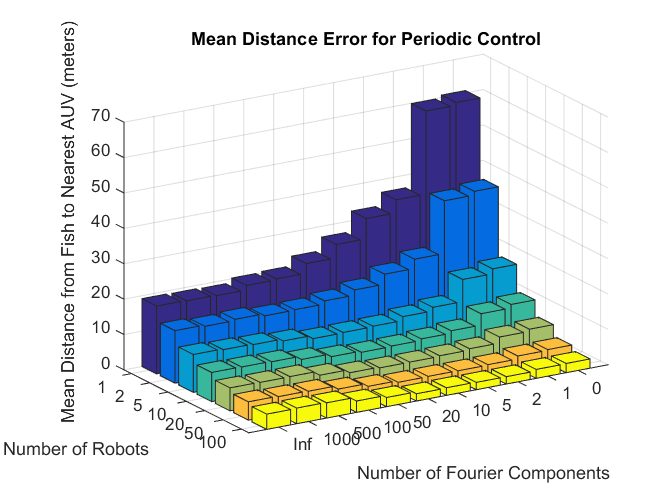
\includegraphics[width = 0.7\linewidth]{results/periodicMeanDistance}
		\caption{The above plot shows the average distance from a fish to the closest AUV when using the periodic control with varying numbers of AUVs and Fourier components.}
		\label{fig:periodicMeanDistance}
	\end{figure}
	\\\\
	Figure \ref{fig:periodicFraction} shows the Fraction In Range error for the periodic control. When 50 or more AUVs are present, regardless of the number of Fourier components used, more than 90\% of the simulated fish remain within range of the AUV. This fraction remains above 80\% when there are more AUVs than there are nodes, as long as 10 or more frequency components are kept. But when the number of AUVs falls below the number of nodes, the fraction of fish within range rapidly drop off to the best case of 35\% in the single AUV trials.
	\begin{figure}
		\centering
		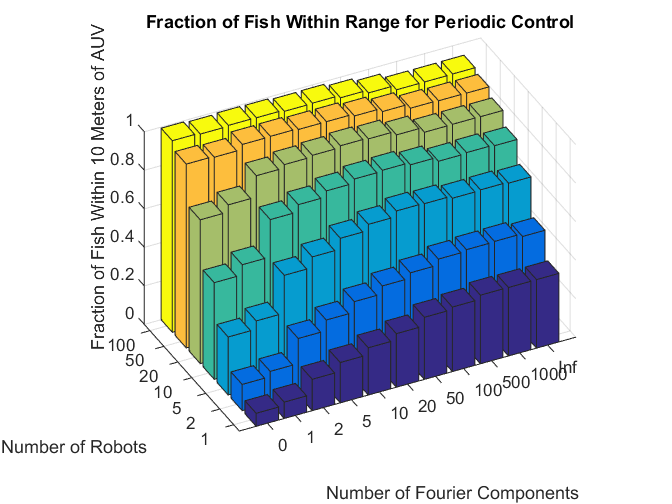
\includegraphics[width = 0.7\linewidth]{results/periodicFraction}
		\caption{The above plot shows the fraction of fish within 10 meters of an AUV when using the periodic control. Note that the independent axes are reversed with respect to the graphs in the other periodic control figures.}
		\label{fig:periodicFraction}
	\end{figure}
	\\\\
	Finally, Figure \ref{fig:periodicDensity} shows the Population Density Error. With 50 or more frequency components and 10 or more robots, this error flattens out between 0.21 and 0.25. The error tends to increase with the number of AUVs, as more AUVs are available to fit the transition model's predicted population density more precisely. Additionally, error tends to decrease as more frequency components are used and the AUV's transition probabilities converge on those of the simulated fish.  
	\begin{figure}
		\centering
		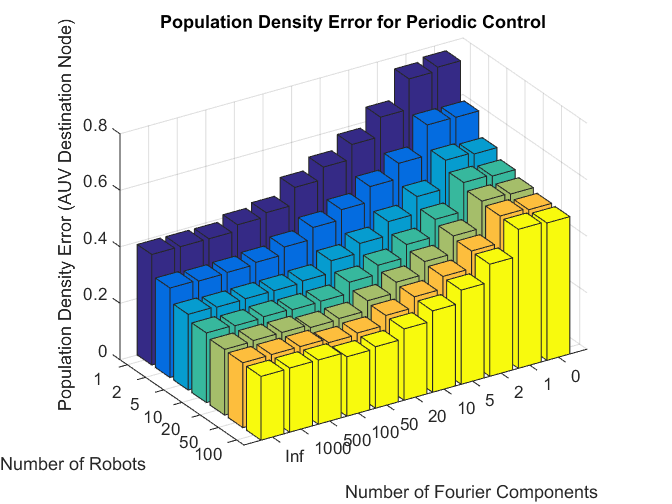
\includegraphics[width = 0.7\linewidth]{results/periodicDensity}
		\caption{The above plot shows the Population Density Error from periodic control simulations.}
		\label{fig:periodicDensity}
	\end{figure}
	
	\subsection{Feedback Control}
	
	The feedback control was simulated with varying numbers of tagged fish, between 0 (resulting in random transitions) and 100; as well as the number of AUVs, also between 0 and 100. Figure \ref{fig:feedbackMeanDistance} shows the Closest AUV Distance error for these parameters. As was the case with the periodic control, if there are significantly more AUVs than there are nodes, the control can perform well even with little information about the fish. Interestingly, after 5 fish are tagged, additional tagged fish have negligible effect on the error (and slightly increase error when only 1 or 2 AUVs are used). Since the simulated fish population in these tests follows the transition model of a single fish, the distribution of fish is unimodal; as such, a single tagged fish is usually sufficient to bring the AUVs near most of the fish.
	\begin{figure}
		\centering
		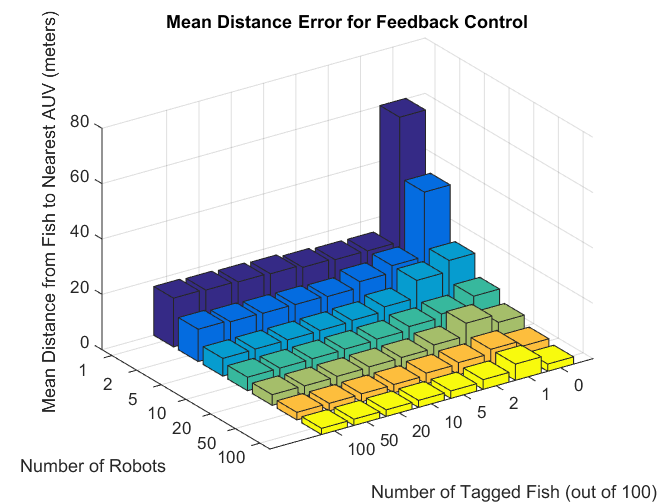
\includegraphics[width = 0.7\linewidth]{results/feedbackMeanDistance}
		\caption{The above plot shows the average distance from a fish to the closest AUV when using the feedback control with varying numbers of AUVs and tagged fish.}
		\label{fig:feedbackMeanDistance}
	\end{figure}
	\\\\
	Figure \ref{fig:feedbackFraction} shows the Fraction In Range error for the feedback control. A striking feature of this plot is the dip in the fraction of fish in range when exactly one fish is tagged. When the number of AUVs significantly exceeds the number of nodes, the random transitions when zero fish are tagged result in a uniform distribution of AUVs across the nodes, resulting in a high probability that all fish will share a node with at least one AUV. But when the number of AUVs is comparable to or smaller than the number of nodes, this random distribution strategy fail to achieve a uniform distribution of AUVs. In this case, the information provided by tagged fish is necessary to best-distribute the limited number of AUVs.
	\begin{figure}
		\centering
		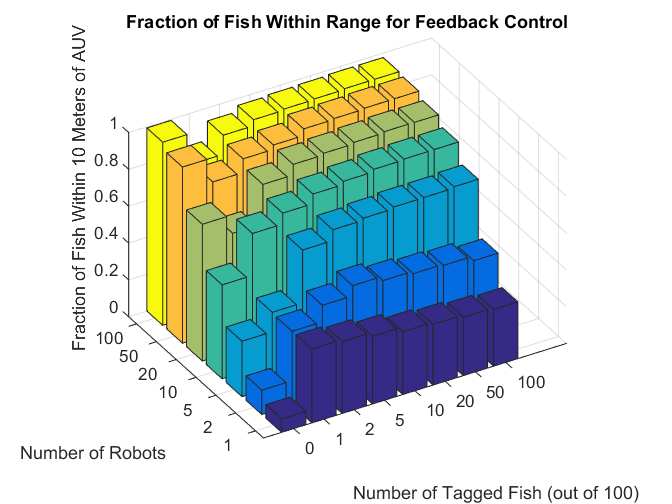
\includegraphics[width = 0.7\linewidth]{results/feedbackFraction}
		\caption{The above plot shows the fraction of fish within 10 meters of an AUV when using the feedback control. Note that the independent axes are reversed with respect to the graphs in the other feedback control figures.}
		\label{fig:feedbackFraction}
	\end{figure}
	\\\\
	Figure \ref{fig:feedbackDensity} shows the Population Density Error. When there are more AUVs than nodes and at least 5 fish are tagged, the error flattens out between 0.10 and 0.13. Again, diminishing returns are evident for tagging more fish; after 1 or 2 fish are tagged, the benefit of additional tagged fish is minimal. In fact, the Population Density Error plot reveals another interesting trend when fewer AUVs are in use. With one AUV, tagging beyond one fish actually \textit{increases} error, from 0.31 when one fish is tagged to 0.43 when all of the fish are tagged. The same effect is visible after tagging more than 5 fish when two AUVs are in use and after 20 fish when 5 AUVs are used. Increasing the number of AUVs seems to increase the number of tagged fish required to optimize the AUVs' population density.
	\begin{figure}
		\centering
		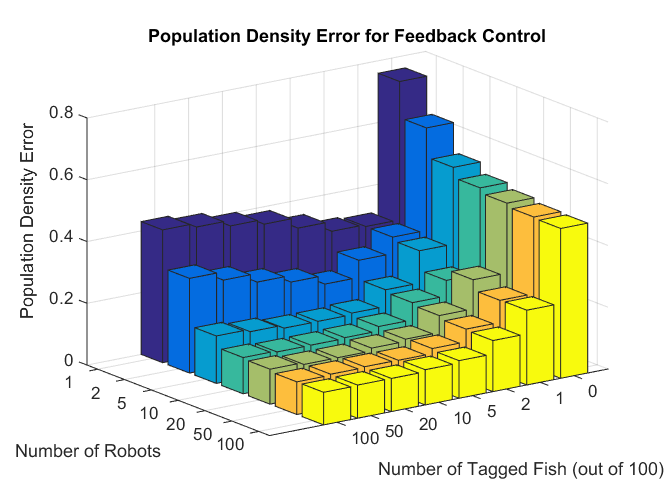
\includegraphics[width = 0.7\linewidth]{results/feedbackDensity}
		\caption{The above plot shows the Population Density Error from feedback control simulations.}
		\label{fig:feedbackDensity}		
	\end{figure}
	
	\subsection{Trends to Investigate}
	
	There are several questions from this data that I wish to investigate further.
	\begin{enumerate}
		\item
		What causes the Mean Distance Error for the periodic control to increase when more than 50 Fourier components are used? Why does the Population Density Error increase when more than 100 Fourier components are used? Why is this increase visible after the same number of Fourier components in both error metrics?
		\item
		Can the spike in feedback control error when one fish is tagged and many AUVs are deployed be quantified?
		\item
		Feedback control error is increased when more fish are tagged and few AUVs are present, but decreased when more fish are tagged and many AUVs are present. Can this relationship be quantified? What theorems from statistics can be applied here? 
	\end{enumerate}
	

	
\end{document}